\documentclass[UTF8]{ctexart}

\usepackage{algorithm}
\usepackage{algorithmic}
\usepackage{amsmath,amssymb}
\usepackage{booktabs}
\usepackage{geometry}
\usepackage{tikz}
\usepackage{color}
\geometry{a4paper,scale=0.7}


\begin{document}
    李青航 SA22225226

    \noindent\textbf{325}

    特征方程$x-4=0,~~~~x=4$

    所以齐次通解 $c_1 4^n$

    设非齐次特解 $an\cdot 4^n$

    又有$h_0=3,~~~~h_1=4\times 3+ 4=16$

    有
    \begin{equation*}
        \begin{cases}
            c_1=3\\
            c_1\cdot 4 +a\cdot 4= 16
        \end{cases}
    \end{equation*}

    得$c_1=3,~~~~a=1$

    所以$$h_n=3\cdot 4^n +n\cdot 4^n$$

    ~\\
    \noindent\textbf{331}

    \begin{equation*}
        \begin{aligned}
            g(x) =& \sum_{n=0}^{\infty} h_n x^n\\
            =& \sum_{n=0}^{\infty} \binom{n}{2} x^n \\
            =& x^2\sum_{n=2}^{\infty}\binom{n}{2}x^{n-2} \\
            =& x^2\sum_{n=0}^{\infty}\binom{n+2}{2}x^{n} \\
            =&  \frac{x^2}{(1-x)^3}
            \end{aligned}
    \end{equation*}

    ~\\
    \noindent\textbf{341}

    $$h_1(x)=h_3(x)=1+\frac{x^2}{2!}+\frac{x^4}{4!}+\frac{x^6}{6!}+\dots=\frac{e^x+e^{-x}}{2}$$

    $$h_5(x)=h_7(x)=h_9(x)=\sum_{n=0}^{\infty}\frac{x^n}{n!}=e^x$$

    \begin{equation*}
        \begin{aligned}
            g^{(e)}(x)
            &=h_1(x)h_3(x)h_5(x)\dots h_9(x)\\
            &=\biggl(\frac{e^x+e^{-x}}{2}\biggr)^{2}\cdot e^{3x}\\
            &=\frac{e^{5x}+2e^{3x}+e^x}{4}\\
            &=\sum_{n=0}^{\infty}\frac{5^n+2\cdot 3^n+1}{4} \frac{x^n}{n!}
        \end{aligned}
    \end{equation*}

    所以$$\displaystyle h_n = \frac{5^n+2\cdot 3^n+1}{4}$$

    ~\\
    \noindent\textbf{343}

    将圆上的点划分为两部分(这两部分连续),第一部分有$2k$个点,第二部分有$2n-2k$个点,
    总的方法数$$h_n=\sum_{k=1}^{n-1}h_{k}h_{n-k}~~~~n\ge 1,~~~~h_0=h_1=1$$

    所以由凸多边形三角剖分的例题知,解就是卡特兰数

    $$h_n = \frac{1}{n+1} \binom{2n}{n}$$


    ~\\
    \noindent\textbf{346}
    见图
    \begin{figure*}[h]
        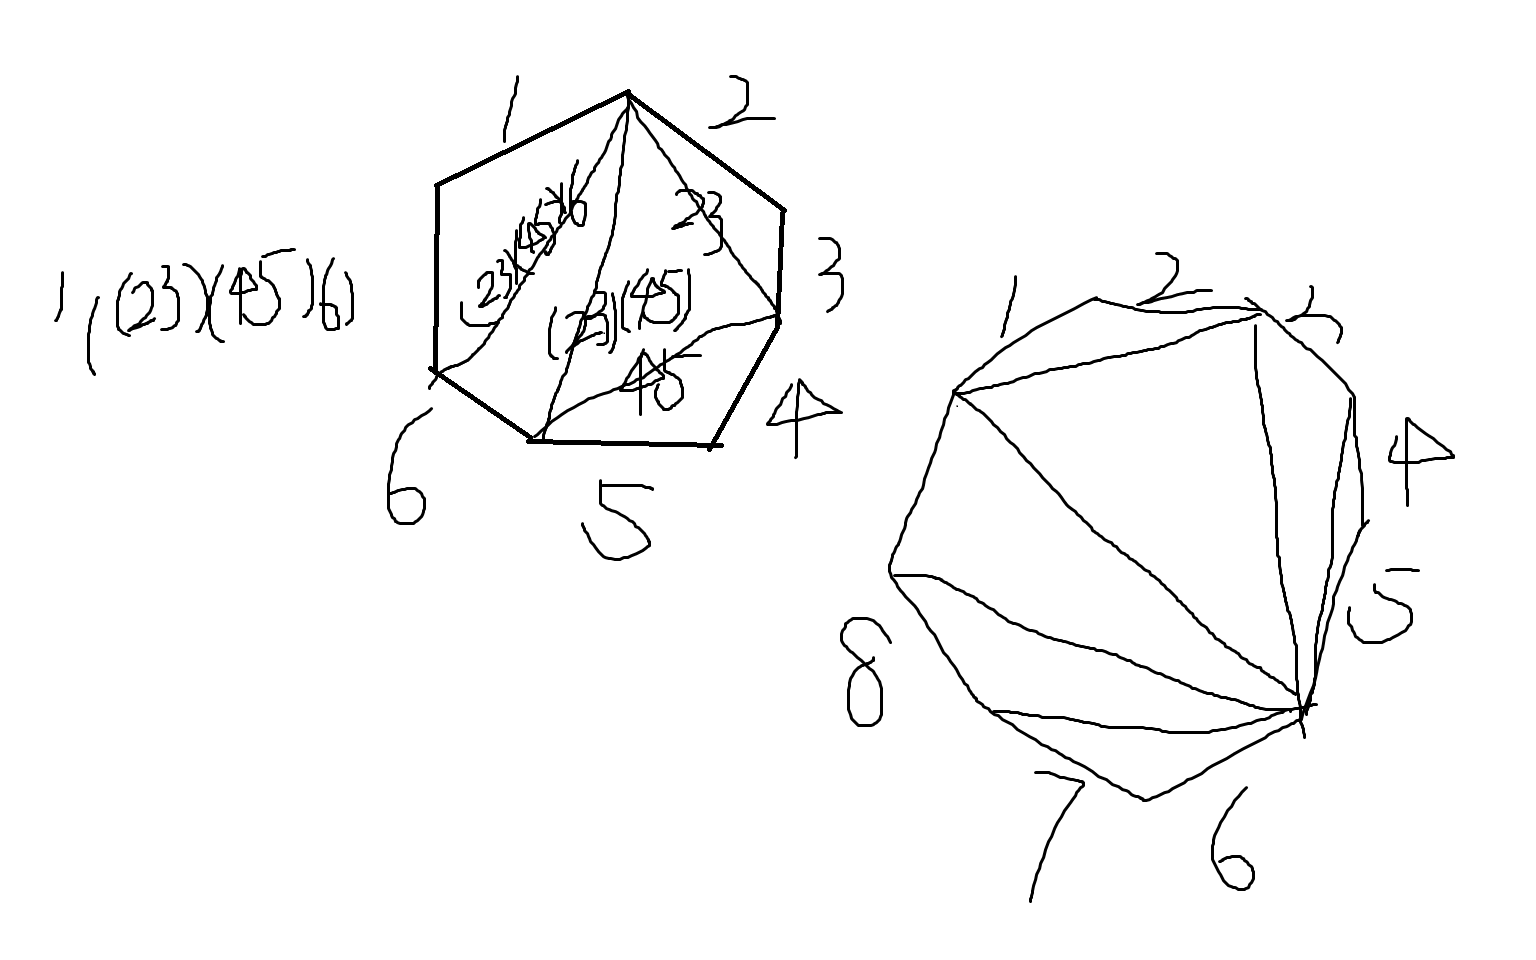
\includegraphics[width=1\linewidth]{1.png}
    \end{figure*}

    ~\\
    \noindent\textbf{348}
    $$h_n = 2n^2 -n + 3$$

    差分表

    $$3, 4, 9, 18, 31, 48, 69, 94, 123, 156\dots$$
    $$ 1, 5, 9, 13, 17, 21, 25, 2, 33\dots$$
    $$4, 4, 4, 4, 4, 4, 4, 4\dots$$
    $$ 0, 0, 0, 0, 0, 0, 0\dots$$

    所以$h_n = 3 \binom{n}{0} + \binom{n}{1} + 4 \binom{n}{2}$,进而

    \begin{equation*}
        \begin{aligned}
            \sum_{k=0}^{n} h_k =& 3 \sum_{k=0}^{n} \binom{k}{0} + \sum_{k=0}^{n} \binom{k}{1} + 4 \sum_{k=0}^{n} \binom{k}{2} \\
            =& 3 \binom{n+1}{1} + \binom{n+1}{2} + 4 \binom{n+1}{3} \quad n \ge 0
        \end{aligned}
    \end{equation*}

\end{document}